\clearpage
\chapter{System implementation}\label{ch:implementation}
\begingroup
\clubpenalty=10000
\widowpenalty=10000
\brokenpenalty=10000

The implementation follows the patient state from MRI inputs to anatomical and image outputs. Encoders build a compact visit vector, a spatial feature grid, or a hierarchy of feature maps. We keep readouts and temporal predictors separate from these encoders so that each can be tested while the others remain fixed.

\section{Preparing images and longitudinal batches}

The BrainIAC input pipeline applies N4 bias-field correction, isotropic resampling and brain extraction before preparing a 96 × 96 × 96 array. Rigid registration uses an MNI template when one is supplied. Nonzero intensity normalization computes the mean and standard deviation over the image foreground, keeping background voxels out of those statistics. We retain the pre-resize geometry for physical measurements: anatomical volumes come from source masks, while the resized arrays provide network inputs.

The longitudinal batch arranges MRI by patient, visit and sequence. Padding gives patients with different numbers of visits a common tensor shape. A visit mask identifies real visits, and a sequence-availability mask identifies loaded images. The image encoder processes the available sequences, and a JEPA prediction pair requires MRI at both its observed and target visits. Clinical features are encoded separately before fusion; treatment-status regressions use the status recorded at the cutoff session as an input distinct from response-assessment labels.

\section{JEPA encoding and temporal prediction}

The compact image encoder is a three-dimensional Vision Transformer initialized from BrainIAC weights \cite{ref16}. Each sequence produces a 768-component vector. We average the available sequence vectors to form a visit representation, so its size stays fixed when a sequence is missing. Low-rank adaptation updates small parameter matrices in selected linear layers while the base weights remain frozen.

For multimodal prediction, we normalize the clinical and image features and concatenate them into a visit token. We add timing encodings before passing the tokens to the temporal Transformer. At a given cutoff, the Transformer receives only the prefix ending at that visit. The output at the last real visit becomes the temporal state; the visit mask keeps padding out of the attention calculation.

A multilayer perceptron maps this temporal state into the target feature space. The target encoder is a copy of the image backbone and projection head, updated through an exponential moving average of their parameters. It runs in evaluation mode without gradients, providing a slowly changing target as the online encoder learns. The prediction loss is one minus the cosine similarity between normalized predicted and target features.

Figure~\ref{fig:5.1} shows how the two paths meet at the loss. Anatomical readouts then map the learned representations to compartment volumes, making the forecast interpretable in the same units as the anatomical targets.

\begin{figure}[!htbp]\centering
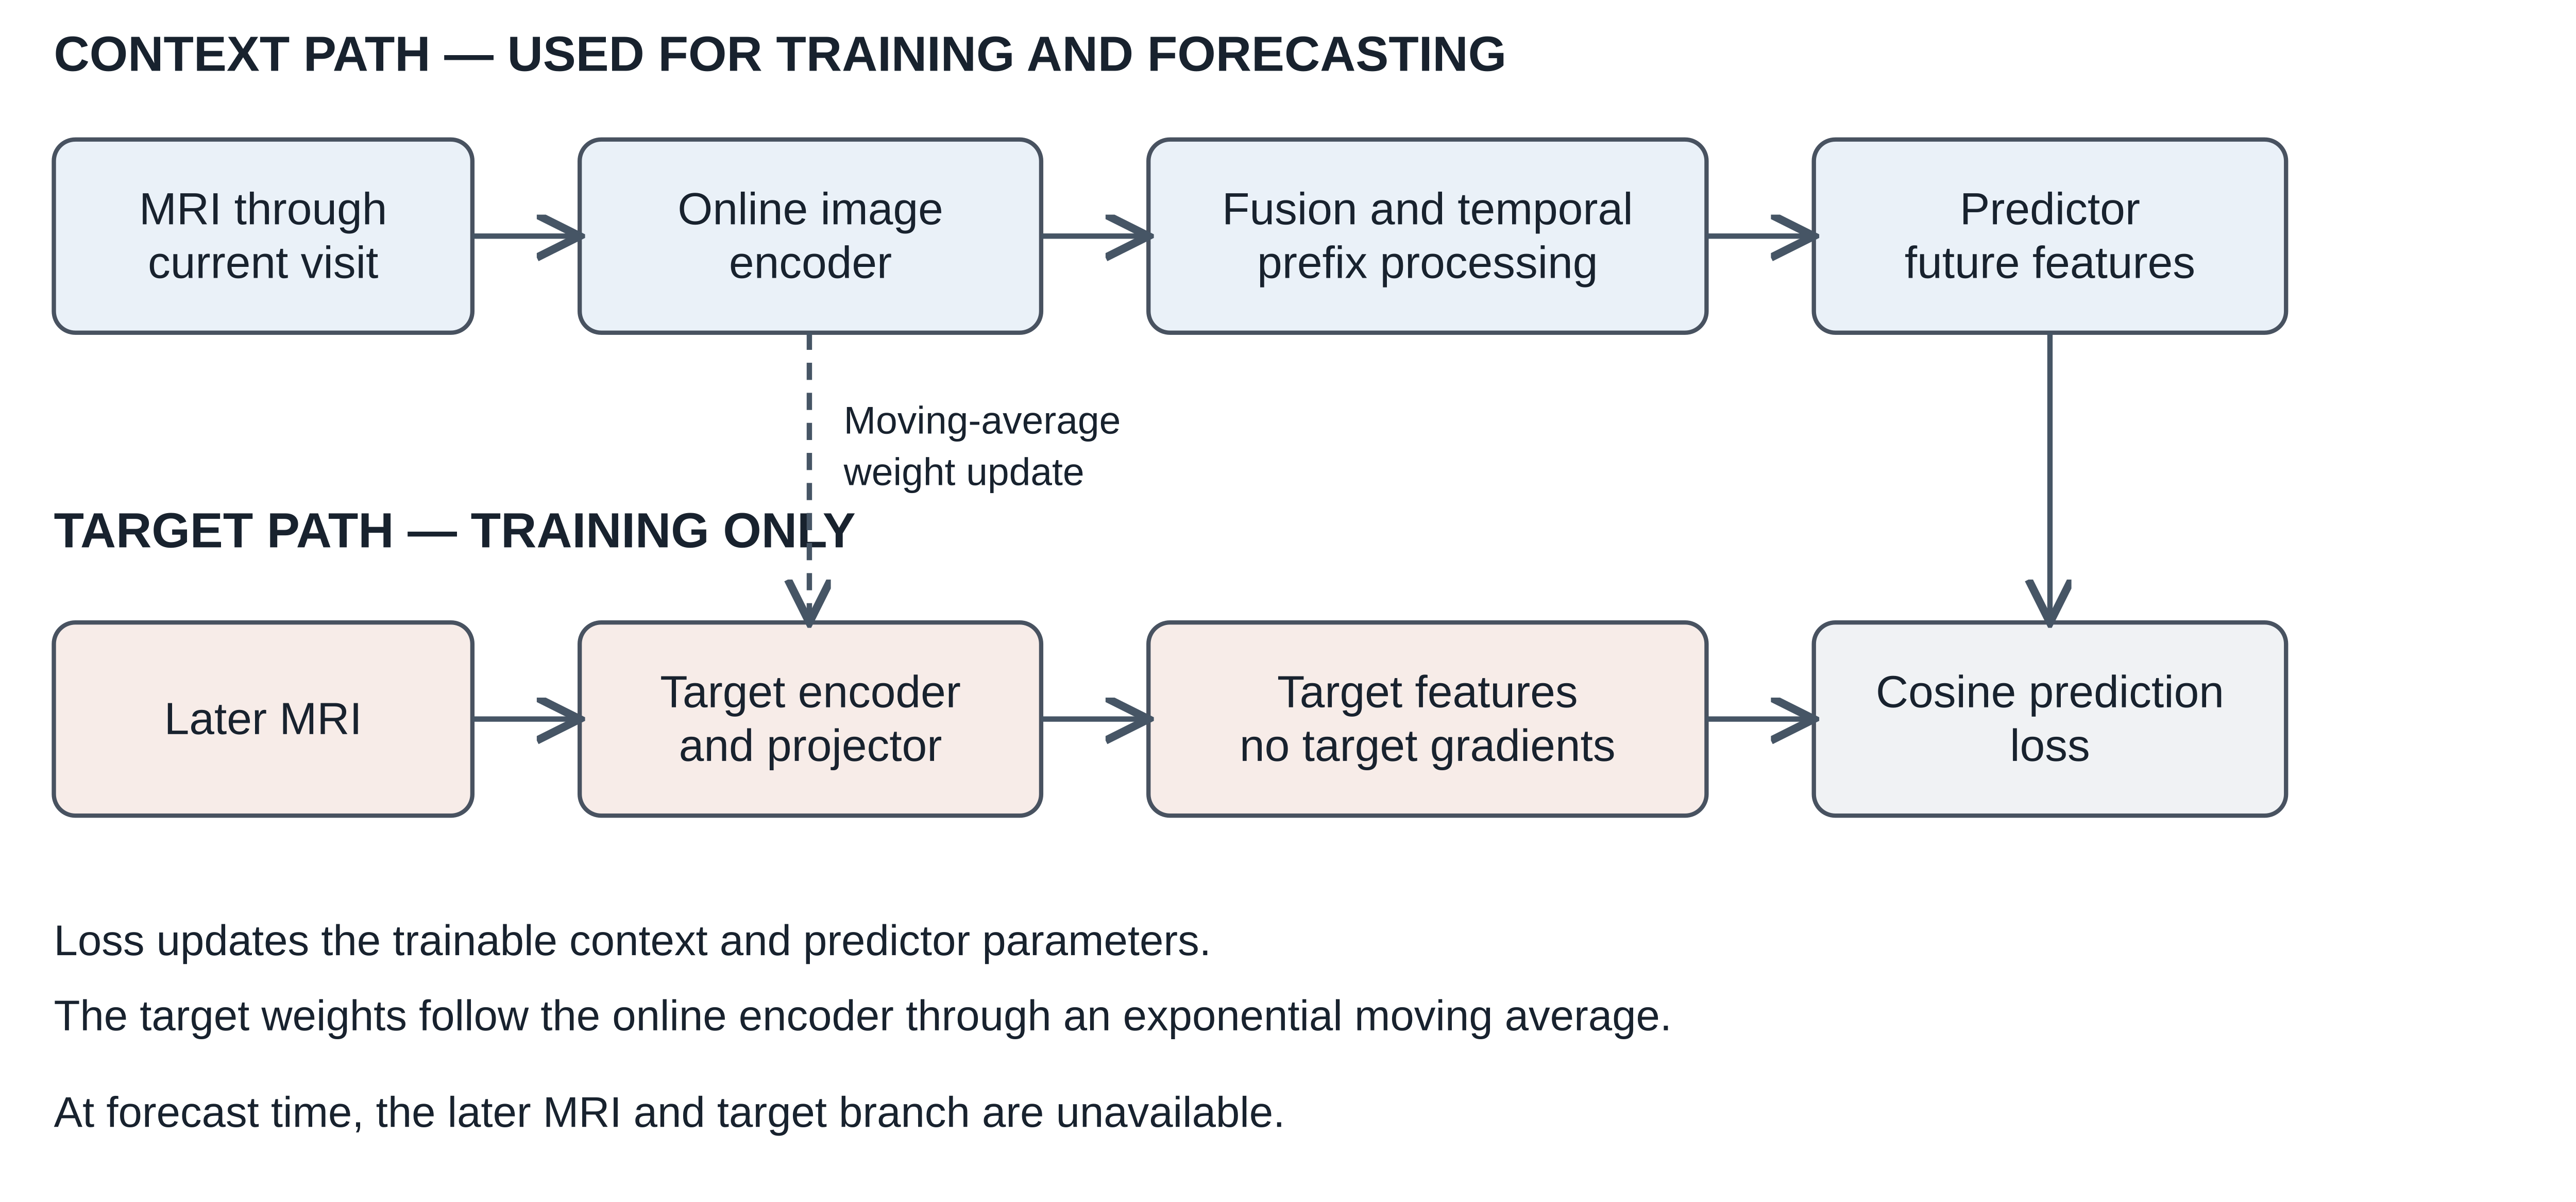
\includegraphics[width=\linewidth,height=0.57\textheight,keepaspectratio]{figures/figure_5_1.png}
\caption[JEPA training paths and the context path retained for forecasting]{JEPA context and target paths. The target encoder and projector follow their online counterparts through a moving-average update.}\label{fig:5.1}
\end{figure}

\section{Spatial states and anatomical readouts}

The convolutional spatial encoder receives four MRI channels and four sequence-availability channels. Its residual three-dimensional blocks have widths of 16, 32, 64 and 128. A decoder combines their spatial maps to predict three compartment masks, while spatially averaged features feed a three-output volume head. Binary cross-entropy and Dice loss train the masks; absolute error on standardized log-volume targets trains the volume readout. For observed-change prediction, a paired model processes two available scans. The independent-state control instead subtracts their separately estimated volumes.

The spatial-token encoder keeps a different form of state. It retains the Vision Transformer's sequence-specific tokens on a 6 × 6 × 6 grid, fuses them into 64 channels, and decodes masks at 24 × 24 × 24. This preserves spatial inputs to the readout instead of reducing each visit to one vector. Pretrained and random versions share the architecture, supervision, training draws and initial non-backbone weights, with all encoder parameters trainable. Their comparison therefore changes initialization while keeping the decoding problem fixed.

The integrated observation model retains higher-resolution encoder maps alongside the compact state. Both its anatomical decoder and its missing-sequence decoder read these saved features. Cavity supervision covers the full annotated field, including labeled cavity outside the MRI foreground, while image losses use the MRI foreground. Keeping those supports separate allows the anatomical loss to include all annotated tissue without filling the image objective with background voxels.

\section{Completing and predicting FLAIR}

The token-based completion model predicts current FLAIR from CT1, T1 and T2. BrainIAC supplies all 216 spatial tokens for each sequence. A fresh head projects their concatenated features to 64 channels and upsamples the 6 × 6 × 6 grid through convolutional blocks to 96 × 96 × 96. We fit the same head with either an adapted encoder or the original frozen encoder to test what completion training adds to the representation.

For future-image prediction, each encoder is frozen and receives fresh matched forecast heads. A recurrent unit combines non-FLAIR tokens across visits at each spatial location. The decoder predicts an image residual that is added to the latest observed FLAIR. This gives the model a direct persistence path and leaves it to learn the correction. History and latest-only heads share that path and the same past timing; earlier FLAIR is excluded from the history representation. Completion and forecasting both minimize image MAE in a fixed field derived from fitting-patient T1 images.

\section{Predicting change in spatial features}

The frozen-state predictor holds the anatomical encoder and volume head fixed while learning how their state changes. It reduces 128-channel maps to a 16-channel recurrent state and processes up to four visits with a convolutional gated recurrent unit. Past gaps and sequence-availability flags enter alongside each map. A residual head predicts a correction to the latest map, and a scale head produces 128 positive uncertainty scales.

The frozen affine volume decoder converts the predicted feature means and scales into Gaussian log-volume distributions. Training minimizes anatomical CRPS plus 0.1 times standardized feature-mean squared error. The anatomical term connects the prediction to the quantity being evaluated, while the feature term keeps the predicted state tied to the encoder's representation.

We implement the history controls by changing the earlier maps at the predictor input. Latest-only replaces them with zeros but retains their timing, availability flags and visit mask. Pooled history replaces each earlier map by its spatial mean. These changes distinguish the contribution of earlier images from the contribution of their spatial detail.

Gradient routing determines whether the state itself can adapt to forecasting. Joint training lets forecast losses update the encoder. Observation-only training detaches the encoder from forecast losses while continuing to train its current-anatomy readouts. The supplied-horizon variant adds the realized week-bin interval to both history and latest-only predictors and compares spatial recurrence at two resolutions.

\section{Forecasting from anatomical measurements}

Ridge regression provides a forecast directly from anatomical quantities. Treatment-status models use saved volume estimates from the spatial encoder, adding the preceding state difference for history and current treatment status with its state interactions. Inner patient folds select the ridge penalty and estimate residual uncertainty; outer folds provide predictions for patients outside that fit. Measured-state models use whole-compartment reference volumes, with horizon-aware variants adding the supplied interval and interactions with current volume and prior velocity.

Regional models use source-mask measurements. Each labeled voxel contributes its physical volume to the region containing its center. The implementation records out-of-field volume separately so that regional and outside totals can be checked against the source total. Eight regions give 24 region-compartment values for LUMIERE and 32 for MU-Glioma-Post, which includes cavity.

The numerical predictors comprise persistence, mean change, constrained trend extrapolation, current-only ridge, history ridge and shuffled history. Current-only ridge uses current measurements and the past gap; history adds the previous measured change. We standardize features using fitting patients, giving each patient equal total weight. The ridge penalty is selected from 0.01, 0.1, 1, 10 and 100 by minimum selection MAE. Predictions are clipped at zero because volumes cannot be negative. Each cohort has its own fitted coefficients and normalizers.

\section{Structured anatomy and quantity models}

The structured forecaster represents possible futures as anatomical scenarios. It conditions spatial changes on current images, predicted anatomy and, in the history version, the previous observed change. Current volumes, timing and the requested horizon determine scenario coefficients and mixture weights. Each scenario supplies a segmentation and the volumes measured from it, keeping its shape and burden consistent. Scalar controls predict volume distributions from the corresponding current or historical quantities.

The quantity model separates compartment presence and amount from spatial allocation. It fits presence and voxel counts, constraining each count by the remaining available voxels and reserving space for later compartments sampled as present. Exact discrete cumulative distributions provide deterministic core mean-volume and CRPS scores. This lets us assess the fitted quantity distribution directly, without making its score depend on a small sample of anatomical scenarios.

\section{Selecting another MRI sequence}

The acquisition model uses a shared sequence encoder and order-independent fusion: the same observed sequences produce the same state regardless of reveal order. A hypothetical-feature predictor estimates the representation of a candidate sequence. Matched ridge selectors use features of the observed state, with the JEPA selector receiving an additional block of predicted candidate features and the direct selector using zeros in that block.

When a sequence is revealed, its actual MRI updates the observed state. The anatomical and completion decoders then read the updated features. Hypothetical features guide the choice of sequence, while the saved observation state contains the features of images actually received. This keeps the acquisition decision connected to the same readouts used to assess the representation.

\section{Training and restoring the models}

The JEPA trainer uses AdamW with learning-rate warmup and cosine decay. Mixed precision, chunked image encoding and activation checkpointing reduce memory use. Gradient accumulation combines several small batches into one optimizer update. In pair-weighted accumulation, each batch contributes according to its valid prediction-pair count. The learning-rate schedule and moving-average target update advance with optimizer steps, so their rate of change follows parameter updates rather than individual batches.

Checkpoint selection follows the output being learned: anatomical CRPS for probabilistic forecasting, nonempty-compartment Dice for the matched anatomical encoder, and image MAE for completion and image prediction. The frozen-state forecast also selects an uncertainty multiplier on selection patients. Ties retain the earlier checkpoint, and numerical regressions choose their penalties before final scoring.

Saved checkpoints contain model parameters, optimizer state, epoch and configuration. Evaluation restores the fitted normalizers and readouts with the weights because all three determine the prediction. Stored features retain patient, visit and encoder identities so that competing predictors can use the same observations. Chapter~\ref{ch:testing} describes the checks that saving, restoring and scoring these components reproduce their outputs.

\endgroup
